\chapter{Disciplinary Implications} 
\label{ch:experiments}

\section{Implications of the pandas Case Study}

As discussed in the Integration chapter, pandas was chosen for the case study in applying the Concepts chapter concepts because pandas is an active repository with an involved, well-organized development community who uses the full extent of possible tools in the repository. A case study was necessary for this thesis research because it would be best to apply the library concepts in a qualitative manner, as this allows for in-depth discussion of the details of the values and actions from the Concepts chapter to test why and why not they apply to a Github repository, Github itself, and a FOSS community associated with the repository. This also creates an opportunity to test the practical application of the new interdisciplinary glossary terms which resulted from the Concepts discussion. 

\subsection{Excluded Library Values}

As a result of the pandas case study, it is necessary to explore the implications of this in terms of the concepts (library values, actions of the CCAL, code literacy, peer-to-peer networks) and the practical application of the interdisciplinary glossary terms. Nine of the library values and library and information science values applied to the pandas repository, excluding Equity of Access, Democracy, Reading and the Book, Justice, and Aesthetics \cite{gorman2000values}\cite{rubin2016foundationslis}. These values do not apply to Github and the pandas repository in a way which preserves the meaning of the value. However, because the value does not apply to pandas or Github does not mean the value could not apply to any Github repository. There may be repositories which a value applies to the project or community, however it is not possible due to the scope of the thesis to apply qualitative study to further repositories. Therefore, there is an opportunity for future work in applying these values to study other repositories. 

Some values, such as Democracy, are difficult to apply to Github or apply to understand ways in which Github could be included in the physical library \cite{gorman2000values}. Especially given the decentralized nature of Github and the success of the current organization of FOSS community, it is difficult to suggest ways in which Github could improve to better align with Democracy. However, Equity of Access, Reading and the Book, Justice, and Aesthetics can be applied in ways beyond the Github repository. 

Equity of Access is complicated in applying to Github because Github requires an electronic device to access, and a computer with a CLI to contribute to repositories using Git\cite{gorman2000values}. However, this could be addressed by more efforts to include libraries in code literacy efforts and library computer labs being a point of access to Github. However, having these labs as an access point for individuals without wifi or a computer in their living space does not create total equity with the individuals who do have these resources in their living space. A more equity-focused approach might be loaning laptop and wifi router programs or expanding these programs if they already exist. This is similiar to Rubin's value of Justice, which also did not apply by definition in the pandas case study \cite{rubin2016foundationslis}. In the Concepts chapter, it is noted that the Github Docs do not discuss fairness in access to the platform. Because access to the necessary wifi and technology could impact a user or contributor's access to Github. Perhaps Github Docs or repository Wiki tabs, both being sources of information, could hep link users to their nearest local library and loaning laptop/wifi programs if those programs exist. 

A major factor of Reading and the Book is advocating for literacy \cite{rubin2016foundationslis}. When considered in more interdisciplinary terms including Computer Science, as discussed in the Concepts chapter, the value of Reading and the Book could be applied for the literacy of code. With this understanding and the importance to society of literacy of code argued by Vee, it implies that libraries have an opportunity to become more involved in supporting code literacy efforts since this has become a legitimate literacy and therefore aligns with the LIS value of Reading and the Book \cite{vee2017coding} \cite{rubin2016foundationslis}. 

As discussed in the Concepts chapter, Aesthetics already applies to the Github Archive Boxes \cite{githubarchiveboxes}. There are two potential implications of this connection. The first to is further expand this program from a LOCKSS perspective and create more boxes with the same important repositories held within \cite{githubarchiveboxes}. Second, this program could extend into preserved forms other than the film in the current boxes \cite{githubarchiveboxes}. Perhaps there is another form this archive could take on, or multiple, which are more accessible to work with interactively than film, where it might be easier to read the code and navigate the repositories with a full understanding of their structure. 

\subsection{Excluded CCAL Actions}

In addition to the library concepts which did not apply to pandas in the case study, there were CCAL actions which did not apply. These were Responsible Custody, Advocacy, and in some cases Diversity \cite{rubin2016foundationslis}. As discussed in the Concepts chapter, the application of Responsible Custody is complicated by the individual choice to participate in FOSS communities. A maintainer could leave the repository community at any point, or not work on a project for an extended period of time. When the maintainer abandons a project, they are not under a requirement to pass that repository and maintaining of it to another person. Because they are not under this obligation due to the nature of FOSS contribution and communities, Responsible Custody could not apply to Github unless the maintainer did pass it on. This action could still be considered for other repositories as future work, but it did not apply to pandas because this is an active repository with multiple maintainers who are very involved in contributing often \cite{pandasrepo}. 

As also discussed in the Concepts chapter, the action of Advocacy does not apply to Github in the current moment other than potentially if prior versions of the repository are used. It is not possible to track through the repository which versions of the software is being used by users. In pandas, previous versions of the software are recorded as Releases, but again there is not way to track when prior versions are being downloaded to peer repositories. Because of this, there is an opportunity for Github to record the number of downloads for each release of a project as a loose application of Advocacy. This could also be a quantitative way of showing the historical value of previous releases, which asserts the application of History and Memory \cite{rubin2016foundationslis}. 

It is important to note the application of the CCAL action of Diversity to pandas differs slightly from the given definition. Diversity as it applied to pandas applied to the way in which Github makes record of all contribution (commits, issues, PRs), therefore this part of the definition applies: "Archivists collectively seek to document and preserve the record of the broadest possible range of individuals, socioeconomic groups, governance, and corporate entities in society" cite\cite{rubin2016foundationslis}. However, the next part of the definition does not apply directly to pandas, Archivists embrace the importance of identifying, preserving, and working with communities to actively document those whose voices have been overlooked or marginalized...Archivists accept and encourage a diversity of viewpoints on social, political, and intellectual issues, as represented both in archival records and among members of the profession" \cite{rubin2016foundationslis}. This is because the CCAL action of Diversity is a carried out by Github, and Github is not directly working with individuals and groups who have been marginalized to specifically archive their work, and Github does not actively encourage a "diversity of viewpoints", although Github would still accept record of such viewpoints discussed on the platform \cite{rubin2016foundationslis}. Therefore, the distinction is necessary to note this difference in the definition and application of Diversity in the pandas case study. This also implies that Github is in a position to work with people and communities who have been marginalized, and to take a more active stance in encouraging differing viewpoints. Due to the decentralized nature of repositories, these implications may also apply to the maintainers of repositories.

\subsection{Implications of Applied Values and CCAL Actions}

Overall, the majority of values of both Library Science and Library and Information Science apply to Github based on the pandas case study. As a result of this successful application, there are two implications. The first implication is that Github and its repositories function as libraries, which Github being the Shell Library and the repositories being the Content Libraries. This is because Github holds the repositories yet also takes on library values, and the repositories hold the vast majority of content on Github. As a result of this successful application with pandas, it is necessary for case studies to be done with more repositories on Github since this is a qualitative study. The process of application and discuss should be repeated on different repositories to further affirm the application of concepts. 

The successful application of the majority of both values and actions from the Concepts chapter to pandas overall validates that process as a legitimate interdisciplinary method for studying Github repositories from a library and archive-focused perspective. This is a new understanding of how Github, repositories, and FOSS developer communities operate from a humanistic perspective, and one that is interdisciplinary. Therefore, this implies that it is certainly possible and even necessary to be approaching Github and FOSS communities from a Library Science and archival point of view, for the purpose of fully understanding the meaning behind FOSS projects and Git/Github's technical functions. 

\subsection{Implications of Interdisciplinary Glossary Term Applications}

The practical application of the interdisciplinary terms in the pandas case study implies that these terms have a valid meaning which addresses interdisciplinary connections between Library and Computer Science, and that these terms have a place in the process of understanding how Github functions as a library object and who within the realm of Github takes on the actions of the CCAL. These terms take some of the in-depth discussion of concept application and summarizes them into words meant for a practical understanding, for a more cohesive discussion that lifts up these interdisciplinary connections. The validity of this new terminology implies that it should be used again through repetitions of the case study on other repositories. 

The existence and validity of this terminology also implies that it should be released to the Github community so that they may benefit from the use and understanding of it. Because many Library Science masters programs are now also Library and Information Science, it would be beneficial to the discipline for this terminology and the methodology of the case study to be available for the profession as a doorway from Library Science and archival concepts to a digital humanities understanding of a major technical resource in Computer Science. This opens doors not only from Library Science to Computer Science, but from Computer Science to Library Science as well. These terms which apply to developer's communities have the opportunity to create new learning experiences about Library Science for them, thus expanding their understanding of Github beyond a purely technical perspective, encouraging better utilization of to full repository template, and best community interactions.

\section{Interview with Scholars}

Because the of the overall successful application of the CCAL methodology, GCN, and library values to Git/Github, it is necessary to explore and evaluate the implications of the study. This is completed through interviews with scholars, which have been conducted as a means to evaluate the interdisciplinary integration from a high level perspective, and exist in place of the traditional experiment for the thesis to best fit the interdisciplinary nature of this research. Three scholars were interviewed, with two of the interviews occurring over email. The email interviews included three of the five questions. One of the interviews occurred over Google Meet, which included all five questions.

This is a slight change from the planned discussion panel. Invitations to the panel were sent out to librarians, and professors and scholars in the Digital Humanities whose work focuses on libraries and/or technology. The invitation included a short abstract on the topic of the panel, and questions would be sent following a response with an RSVP to attend. After another attempt to reach out to several more invitees when only one of the original invitees had RSVP'd to attend the panel, it was necessary to change the panel to interviews to be able to communicate with more than one scholar in the field. 

\subsection{Overview of Interviews}

The participants for the interviews were Elæ Moss, Tim Ribaric, Cody Hennesy, and Patrick Williams. Moss is a digital humanities scholar who maintains and organizes The Operating System, Ribaric is a Digital Scholarship Librarian at Brock University, Hennesy is a Journalism and Digital Media Librarian at University of Minnesota, and Williams is a Humanities Librarian and the Lead Librarian for Digital and Open Scholarship and Syracuse University. 

The Google Meet interview with Williams was held virtually from 6pm-7pm EST on March 17th. This interview was held on this date to allow for an extensive time to establish the concepts of the thesis and apply these concepts to Github, to allow for questions to be formed for the discussion. All five questions were discussed during this meeting, which were: 

\begin{enumerate}
  \item A concern experts in library science have as technology has become increasingly prevalent is the replacement of books with electronic records. In what ways could the library including code and Github change public perception of the main use of libraries, and how could this be helpful or harmful to libraries?
  \item In practice, given that library science and information science are intertwined, what are the necessary differences between them? 
  \item How often are patrons of the library seeking technology resources specific to computer science, such as written code or instructional resources on how to code, and In what ways is the physical library in its current state equipped and not equipped to provide this education? If this education became a more central mission of the library, would more patrons seek out this information? 
  \item How is the library equipped to catalog the activity and product (finished work, commits, and releases) of FOSS communities? If so, who in the disciplinary structure is doing this work, and if not, would this fall under the role of an archivist? 
  \item How are digital objects in a library cataloged differently and similarly from a peer-to-peer open source software project which changes over time going through the release process in a version control system eg. Git/Github, and how might this understanding be complicated by Github being a mostly public resource owned by a private corporation? 
\end{enumerate}

Questions were sent to Moss, Ribaric, and Hennesy via email within a day of the panel discussion with Williams. They were sent three of the five questions as these three were the most important questions of the five, which were the last three questions in the list above. The questions were formed primarily for understanding the current state and function of the library, specifically the physical library, and the inclusion of Github there, This is because it would be helpful for understanding the library practically to discuss this with expert who are actively working in the field, and to best address the support needed to support Library Science concepts and practical applications. 

\subsection{Discussion of Interview Outcomes}

The interview outcomes will be discussed question by question, beginning with the two of the five questions which were only part of the video interview, followed by the three questions which were asked to all participants. 

\subsubsection{Question 1}

\textit{A concern experts in library science have as technology has become increasingly prevalent is the replacement of books with electronic records. In what ways could the library including code and Github change public perception of the main use of libraries, and how could this be helpful or harmful to libraries?}
\hspace*{\fill}
This question was based on Gorman's concerns about the integrity of information online and the preservation of physical libraries \cite{gorman2000values}. Since this was one of the first two questions, this was only asked to Williams in the interview on Google Meet, and was excluded from the email interviews. 

According to Williams, "large data sets are becoming more important, and data curation is becoming a major skill for all librarians" \cite{patrickinterview}. Williams also raised the issue of the massive amount of electronic data that exists and how to handle this, suggesting that interfaces can be used to address the volume of data, along with understanding the right way to record versions as it is a "curation issue" overall \cite{patrickinterview}. Williams also noted that although archiving is more prepared to handle this, "Github is the most sophisticated" \cite{patrickinterview}. This is true, especially because of how Github is built to function with archiving, the success in application of CCAL actions, and Github actions, which Ribaric specifically references as to why Github is more advanced in archiving FOSS communities itself \cite{timinterview}. Because large data sets are increasing in importance and the interfaces used to build them are built on computer code, although this may or may not change the public perception of libraries, it implies that there should be advocacy for understanding how the interfaces are built, especially since there is a need for them. It may be helpful to patrons, due to the increasing importance of these data sets, to have interfaces associated with them for the purpose of access. Additionally, because Github is already sophisticated in its archival abilities, this implies that Github itself should be included in the library catalog, prioritized over cataloging FOSS communities directly in the library collection. To address the public perception of libraries, based on the response about data sets and data curation being of importance now, information which is data focused in data and technology is influencing the view of the libraries to include technology more. This could be harmful to libraries if it is not addressed and patrons are seeking this, or if it is not balanced with the importance of print books and other resources in the library as Gorman argues for \cite{gorman2000values}. 

\subsubsection{Question 2}

\textit{In practice, given that library science and information science are intertwined, what are the necessary differences between them?}
\hspace*{\fill}

Like the first question, this second one was only asked in the Google Meet interview. Williams specifically mentions the discipline of Information Studies, which is "both discrete and overlaps" with Computer Science and Library Science, as it "accommodates beyond scientific to include creative and design research" and that "human people are very important" in Information Studies \cite{patrickinterview}. There is also Information Science, which is more focused on "underlying technical concepts, less tied to direct use" as it is more focuses on a "universal process" \cite{patrickinterview}. In the interview, we discussed how Information Studies is often the name of the PhD associated with a Library Science program. It is interesting to consider how Information Science verses Library Science and a "creative and design" approach applies to the Github Circulation Network and the methodology of the pandas case study. The Github Circulation Network being founded on Peer-to-Peer principles takes on more of an information science approach, whereas the overall pandas case study approaches the design of the repository and the interactions between contributors from a humanistic library science perspective. Overall it could be argued that the case study as a whole could fall under Information Studies. 


Additionally "there is room for Computer Science in Library and Information Science, for literacy in librarians' work and patrons work in computation" \cite{patrickinterview}. This supports the integration of the disciplines by reaffirming the interdisciplinary nature between the two. The implication of this is that the library must be equipped to address technology and code related question from patrons, and that library programming should support this as well. 

\subsubsection{Question 3}

\textit{How often are patrons of the library seeking technology resources specific to computer science, such as written code or instructional resources on how to code, and in what ways is the physical library in its current state equipped and not equipped to provide this education? If this education became a more central mission of the library, would more patrons seek out this information?}
\hspace*{\fill}

For this question Moss wrote, "I'm interested in creating open access resources including information on things like how to code or use other tech-driven / supported tools...There isn't a physical library, and the digital archive's holdings are not equipped for this though I'd like to see it grow to include more of this sort of support" \cite{elaeinterview}. Because the digital archive is not equipped at the current moment, this indicates that scope is an important factor to consider in the ability for libraries to support computer science-specific and learning to code resources. In a digital sense this would have to do with digital space, but applied to the physical library this implies that the library may require additional personnel who are trained in reference and education for programming and code, rather the training the librarians and workers currently in the library. This would likely best be carried out by an individual who takes on actions and qualities of the CCAL. 

On patrons seeking out this information on computer science resources and written code, an important point Moss made in their response was "There is often a vast chasm between creating resources and folks finding and using them" \cite{elaeinterview}. They also note it would be difficult to predict if patrons would seek out the information \cite{elaeinterview}. Perhaps this chasm could be addressed by efforts within physical libraries to emphasize resources which include written code and are focused on learning to code. This chasm also implies the importance of Gorman's actions of the librarian and actions of the CCAL, specifically Assist and Instruct \cite{gorman2000values}. This chasm has the potential to be practically addressed in the physical library by the role of someone who is focused on advocating for the literacy of code, which applies to the role of the librarian because advocating for literacy is the action of the librarian according to Rubin's value of Reading and the Book \cite{rubin2016foundationslis}. The chasm implies that the patrons of the library would benefit from this person. 

Ribaric, who works in the physical library, notes that patrons seeking computer science specific resources often seek resources within the department, and patrons who are seeking these resources in the library don't have a CS background \cite{timinterview}. Ribaric references one of their library's programs, "We run a series of introductory python workshops that have a very wide audience, I think lots of people are moving towards the idea of coding and are curious about learning about it. The other catch is that you need staff members who know how to program in the Library to provide that kind of support" \cite{timinterview}. They also reference online programs for learning to code, and that the library has the opportunity to have these programs as their own \cite{timinterview}. This opportunity supports that libraries have the opportunity to engage in supporting the literacy of code, since literacy is already part of the LIS value of Reading and the Book \cite{rubin2016foundationslis}. However, as with Moss's response, there needs to be positions in the library for individuals who educate patrons on code literacy. On this, Ribaric notes how their Masters in Computer Science enables them to provide this support, which implies that any individual who takes on this responsibility may be best equipped for this by having prior education in Computer Science specifically. 

Hennesy noted that there was not data on patrons seeking coding resources, but that it is the library's responsibility to give those resources to patrons \cite{codyinterview}. According to Hennesy, "We collect materials related to programming to support the CS dept needs, for example, but we also teach workshops on computational methods that are open to all"\cite{codyinterview} and "A lot of individuals in the libraries also co-teach computational topics in other settings" \cite{codyinterview}. Due to the seemingly somewhat interdisciplinary nature of this programming and education, it implies that cdoing education in the library setting, although coding being a huge part of computer science, should be approached in an interdisciplinary manner. Hennesy, like Ribaric said and Moss's notes on the "chasm" implies, said that a person helping patrons seek out coding education would allow the patrons to seek out the information more as the question asks \cite{codyinterview}. This once again affirms that there should be a position in the library focused on the literacy of code, directing patrons to those resources and running programming for them. Because, according to Hennesy, this responsibility is shared among multiple people in the University of Minnestoa libraries, it may be that the responsibility exists as an action like those of the CCAL which can be carried out collectively by many individuals or carried out by one person \cite{codyinterview}. 

For this question, Williams said "visibility helps, through posters, artwork, and interactivity", and also how the needs of patrons might be "serviced in specific libraries, such as a Computer Science library" \cite{patrickinterview}. This would make sense, as patrons would be inclined to seek out information that they are aware exists, once they are aware of it. For interactivity, Williams specifically references the Digital Scholarship in the Syracuse Library, which includes "VR development and research" \cite{patrickinterview}. Although this may not be directly "learning to code", this is still a point of interactivity in a library with innovative technology, and certainly has potential to spark interest in learning to code and more about programming in general. An interesting point Williams made was that "licensing becomes an issue to access", as licensing for software, especially proprietary, has limitations \cite{patrickinterview}. Because of this, it may be important for libraries bringing in software to prioritize open source and open access as much as possible to lift the burden of work that occurs when a license presents limitations. Lastly, Williams noted the "importance of traditional library work" and how "there is not a curatorial sense around it yet" in regards to the use of technology and programming being part of the library" \cite{patrickinterview}. This opens the doors to the potential of a separate position in the library focused on this work, to allow for "traditional library work" to continue without interruption and for code literacy efforts as discussed to be given more attention.  

\subsubsection{Question 4}

\textit{How is the library equipped to catalog the activity and product (finished work, commits, and releases) of FOSS communities? If so, who in the disciplinary structure is doing this work, and if not, would this fall under the role of an archivist?}
\hspace*{\fill}

According to Moss, "this library project was built to scale, so it's meant to be able to handle different kinds of documents and data in the future" Moss also questions the library project as an "operational repository" and refers to using additional spaces, specifically Github or wikis \cite{elaeinterview}. The scale seems to be important in evaluating how equipped the library is for this interdisciplinary work. On the involvement of an archivist, Moss notes that this is a position they are looking to include in the digital library, but that there is not a disciplinary structure \cite{elaeinterview}. This implies that even if the structure does not currently include an archivist or the structure doesn't exist, there is room for this position to exist, especially with supporting the scale of the library and its scope.

Ribaric raises the idea that the physical library is not currently prepared conceptually or technically to catalog FOSS communities, and that Github is so well prepared that it would be best to simply reference Github \cite{timinterview}. Interestingly, Ribaric also raises the concern of how library science currently does not value technology enough, but that the library catalog search is far more equipped to bring legitimate information to the patron than a Google search \cite{timinterview}. Both this concern and the note on the validity of catalog search results reflects Gorman's concern of technology and the internet \cite{gorman2000values}. Technology should certainly be valued more in libraries since libraries serve society and technology has become so important in daily life, but it is also true that Google search results are far less valid in the information they give than a catalog search in the library. Because the library may not be equipped to handle cataloging FOSS communities itself at the current moment, and how well-prepared Github is to archive information in itself, this implies that the next step toward including code in the library would be having Github as a database in the library catalog alongside others such as WorldCat. If the library becomes more equipped to catalog FOSS communities and projects, which would be ideal from a LOCKSS point of view, then it would be reasonable to catalog the most vital repositories and projects first, like with how Github approached Github Archive Boxes, although it would be better if access of these archives were in a more accessible format for use \cite{githubarchiveboxes}. 

Hennesy mentions a few ways in which the library is equipped to catalog FOSS communities, although this cataloging is not being done at UMN at all, "The Libraries are closely involved in data curation and data management efforts, which often involve documenting and preserving code related to original research data. The Library web services team are also active open source software creators/contributors" \cite{codyinterview}. With the preparation from knowing not only the process of data management and curation, but also the web services team knowing how Github functions and how contribution on Github works, this certainly indicates that some libraries are some level of equipped to catalog FOSS communities and their work.
Since there exists the opportunity for someone to be doing this work, and these are some on the ways in which someone would be begin to gain the knowledge necessary to prepare for doing this work, although there may be limitations as Ribaric suggested, and these limitations may imply that only certain repositories and FOSS communities are archived. 

Williams argud that "software communities are more equipped than the library because they move faster" \cite{patrickinterview}. This is in agreement with Ribaric, who referenced Github actions in response to this fourth question \cite{timinterview}. Williams also noted on cataloging FOSS communities that "this specific action seems more like archival work" \cite{patrickinterview}. This response indicates that if someone was doing this work, their background would need to be in working with archives, potentially rather than having more of a librarianship background. If FOSS projects were to be cataloged, Williams suggested that they might require a "metadata schema with an access point" \cite{patrickinterview}.  

\subsubsection{Question 5}

\textit{How are digital objects in a library cataloged differently and similarly from a peer-to-peer open source software project which changes over time going through the release process in a version control system eg. Git/Github, and how might this understanding be complicated by Github being a mostly public resource owned by a private corporation?}
\hspace*{\fill}

Ribaric notes that this action of cataloging FOSS projects seems to be more focused in Digital Humanities, and that for libraries, "our commitment to open (source and access) lets us share better than for-profit enterprise" \cite{timinterview}. This is certainly true, because at any point, Github as a private corporation could technically chose to put a paywall on Github or require a paid subscription to access repositories. This would hopefully be highly unlikely because Github recognizes the value of open source, but Github being a private corporation gives them the power to potentially take this action. With the library, this would not be a concern (although there may be late fees) because libraries are publicly owned. 

Williams had several answers which could help to address the evolving nature of FOSS projects from a library perspective. The first of these were "pre-print archives and open access publishing, such as manuscripts and pre-peer review papers, then using DOIs to link information" \cite{patrickinterview}. This raised the question of "does each version get a unique identifier?" \cite{patrickinterview}. On Github each commit, issue, and pull request have a unique ID number, and releases have a unique 3 digit number which increases with each release. Therefore, having a unique identifier when it comes to versions of software might be the best practice to align with what has already been established on Github. Williams also discussed linked data because it is possible to "track to conversation around the item" \cite{patrickinterview}. The linked data approach has potential for use in tracking dependencies between different software projects. The discussion of this question concluded with versioning and the use of DOIs, as according to Williams, DOIs are "sometimes/sometimes not human readable", "DOI synatx is not fully established yet", and how DOIs are not yet best practice in the library \cite{patrickinterview}. Because the synatx is not established and DOIs are currently used in software, including DOIs for Github repositories (pandas has a DOI), this implies that DOI syntax should be established and human-readable DOIs should be considered \cite{pandasrepo}. By having human-readable DOIs, this would help with better understanding the information that it holds, and an established DOI syntax would benefit all uses of DOIs, whether in the library or in FOSS projects.

\section{Implications for Computer Science}

First, the thesis implies that there is a new humanistic method for understanding Github repositories and FOSS communities, and this is grounded in Library and Infromation Science, and includes values of archivists as well. The validity of this new methodology, as shown through the pandas case study, implies future repetition of case studies on other repositories in order to understand how they function from a qualitative, humanistic perspective. Based on the interview discussion with Williams, the case study process specifically seems to fall under the discipline of Information Studies, because the case study has human-focsued elements and approaches the Github repository from a design perspective\cite{patrickinterview}. It is important that this humanistic case study methodology exists because it presents a unique perspective that when combined with a technical perspective creates a fuller understanding of how Github and FOSS communities function. This could help enrich the FOSS communities functionality themselves, to be fully utilizing what Github supports in repositories, and opens the doors to the position of the CCAL learning how the information is organized on Github so that it might be added to the library. 

The repetition of the case study also implies the use and application of the Github Circulation Network as a peer-to-peer system for understanding how information is shared across Github. Because such little work has been done in version control systems that are centralized peer-to-peer systems, and most of the work has focused on decentralized systems, future work is implied in understanding centralized peer-to-peer version control systems. Because of the importance of Github to the discipline, the Github Circulation Network and its process are implicated in educating developers about Github. 

DOIs are already used in repositories, such as pandas, but given the conversation with Williams, Github is implicated in making DOIs a best practice for archiving software projects, and there is an opportunity to consider the use of DOIs in repositories. As discussed in the Interviews section, given the Github requires separate version numbers for each release, it might be best practice if each release were also assigned a DOI. It may even be possible to automate this process of assigning DOIs to new releases through Github, however, this might raise issues on if DOIs would be human-readable. 

\section{Implications for Library Science}

Because of the successful application of Library and Information Science concepts to Github through the pandas case study, and how Github is already equipped to archive information well in itself \cite{patrickinterview} \cite{timinterview}, the library is implicated in including Github as a resource alongside databases such as WorldCat. Including Github as part of the library's virtual catalog provides access for patrons to many open source software projects, is a form of including written code in the  library catalog for patrons to better understand something which is important is today's society, and keeps the archival work of Github to Github while having it still be part of the library, rather than attempting to replicate the process which already works on Github locally. 

Due to the responsibility of literacy librarians have and coding now being considered a literacy, the library is implicated in working to support the literacy of code \cite{rubin2016foundationslis} \cite{vee2017coding}. Based on the interview questions, how this is approached may depend entirely upon how equipped each individual library is to handle this work, wether it is shared amoung several people or under one CCAL. It may be helpful for keeping other library work going to have one specific or several specific positions focused on this programming and working to include FOSS projects and communities in the library catalog individually, although this exact work would heavily depend upon the library, seems unlikely to be comparable to Github. However, this work could still be valuable for patrons and for the event that Github introduces paywalls to full access to FOSS projects on the platform, since it is owned by a private corporation and therefore that risk does exist. 

Because DOIs now have the opportunity to be used for FOSS projects, the library is implicated n considering if DOIs should become best practice for the library itself. The library would also then be implicated in considering the syntax of DOIs, as brought up in interview discussion with Williams, and if these would be human readable or not \cite{patrickinterview}. Because human-readable DOIs might help with instances where it is humans organizing the information, such as in libraries, this would be important to consider in determining syntax. This may need to be considered with automated DOIs for software releases on Github, as those might not be human-readable. There could also be differences between the two, with library DOIs having one syntax and software project DOIs having another, although this could raise issues if FOSS projects were individually cataloged in the library. 

\section{Potential Consequences}

The potential consequence of this work from a library science perspective, as discussed throughout the thesis, is the potential for this new implied work in literacy of code and including technology and FOSS more in library programming and the catalog to be seen as more important than the book or the "traditional library work" \cite{patrickinterview}. This is in line with Gorman's concerns, and he argues for the physical library to be preserved as it is without the value of technology overtaking that of the traditional library. Williams also specific mentions how "traditional library work" must continue to occur \cite{patrickinterview}. This must be kept in mind as integration of the disciplines occur, and the respect is given to the separation between disciplines. The library must continue to be able to serve its original purpose, even if that purpose is evolving to include new ones. 

\section{Summary of Results}

\begin{figure}[hbt!]
\begin{center}
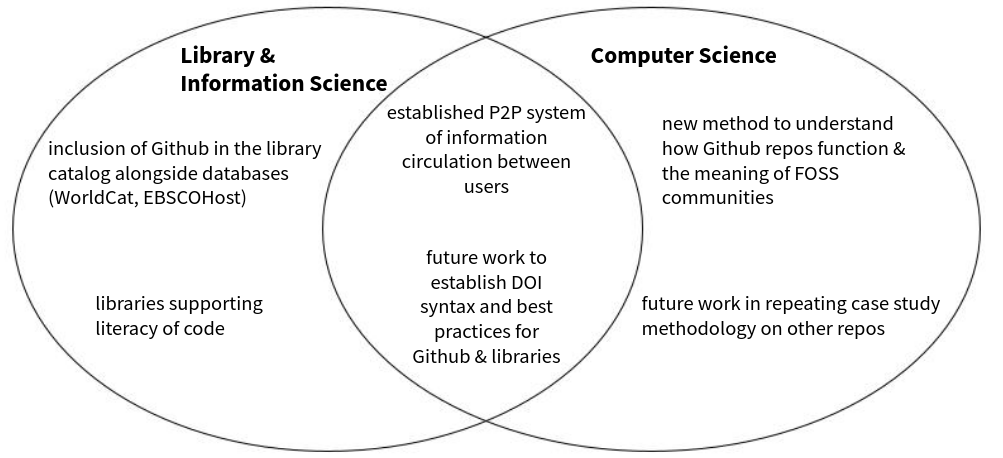
\includegraphics[width=.8\textwidth]{./images/results_venn.png}
\caption{"Venn Diagram to illustrate the outcomes for Library Science, Computer Science, and interdisciplinary outcomes."}
\vspace{0in}
\end{center}
\end{figure}

As a result of this thesis, it is possible and a valid analysis to apply concepts from Library and Information Science to understand the functionality of Github repositories, including the implementation of several new terms which describe the interdisciplinary connections in practical application. This outcome is significant for both Library and Information Science and Computer Science, as it opens the doors to further research. 

\section{Future Work}

Future work beyond this thesis includes repeating the pandas case study using the defined concepts and applying these to other repositories on Github, further study of centralized peer-to-peer systems and how this applies to version control systems, and determining the best practices for use and syntax of DOIs for Github and libraries. The completion of this case study also implies the practical use of approaching repositories in this way, for users of Github/Git, scholars studying the software, and students learning to use Github in a college undergraduate education environment. 

\subsection{Practical Application of Case Studies Methodology}

\subsubsection{Users of Github/Git}

The practical application of the CCAL and the case study methodology for users of Github gives meaning to use of this software, and understanding how the user experience can be best carried out. The decentralized nature of Github and the individual element of choosing to participate in contributing to/maintaining software complicates the practical application of these ideas because they must be communicated to the users. Because this is a specific method that maintainers are not aware of, the practical application would best be carried out by a more broad part of Github, such as Github Education and Github Docs. There is benefit to this being included in Github Education because it already instructs students of the program on how to contribute, so the methods could easily be incorporated in backing up why contributing in those ways are most beneficial. Including this information in the Github Docs may help more experienced users find this information, as they may be less inclined to work with Github Education. 

\subsubsection{Scholars}

For scholars, the case study and CCAL methodology extends into the field of Software Studies, which has been orginally defined by Marino \cite{marino2020critical} and contributed to by scholars such as Vee \cite{vee2017coding}. Although more focused on databases specifically, this also seems to include Ackermans' work \cite{ackermans2020appeal} because their approach to databases is also a critical reading of a software system. Because the CCAL and case study methodologies are interdisciplinary in nature, these systems in a scholarly environment may apply most to scholarship in interdisciplinary fields, such as Software Studies/Critical Code Studies and the Digital Humanities. Future work with these methodologies in a scholarly setting would involve re-applying the methods perhaps with further work in the specifics of reading the repository as a text, or the application of other humanities concepts to repositories alongside or in comparison to the methods defined in this thesis. 

\subsubsection{College Undergraduate Education}

A major component of teaching undergraduate computer science courses is the teaching of best practices for using Github. This covers several levels of computer science education, from learning to write descriptive commit messages in the earliest introductory classes to engaging with the issue discussion and pull request processes in software engineering classes. The methodology of the pandas case study and the actions within the CCAL methodology add meaning to the practical application of these best practises. If the meaning of the best practices were to be taught in addition to the best practices itself, students will have a complete understanding of the importance of best practices. This may lead students to be more inclined to follow best practices, as opposed to if the best practices are taught without the meaning behind them or a simplified meaning that they help with organization or communication alone. In reality, these best practices are upheld by a system that is understood by the methodology of this research. 

